\chapter{Extensibilidad}\label{chapter:extensibility}
Uno de los objetivos de este trabajo es la creación de una herramienta que 
permita la posterior integración de procesos de administración y planificación 
que se llevan a cabo en la Facultad de Matemática y Computación de la Universidad
de La Habana. 
En este capítulo
se presentan la organización y estructura del proyecto, 
se explican algunos detalles de implementación y 
se propone una guía de cómo agregar nuevos 
procesos al sistema.

En la sección \ref{cap5:structure} se presenta la distribución de las 
carpetas de los proyectos cliente y 
servidor, y se describen algunas de las herramientas implementadas que se pueden 
reutilizar en otros procesos que se deseen agregar al sistema.
En la sección \ref{cap5:recommendations} se proponen las pautas y pasos 
a seguir para incorporar nuevos procesos al sistema.

\section{Estructura del cliente y servidor}\label{cap5:structure}
El desarrollo en el lado del servidor se llevó a cabo con el  
uso de la biblioteca Django, en particular Django Rest Framework.
Para el desarrollo de los procesos de asignación de docencia y planificaciones de las 
tesis se crearon dos \textit{apps} independientes de Django, con el objetivo de agrupar los ficheros 
necesarios para la modelación de cada proceso. 
En la figura \ref{img-server-structure} se muestra cómo está estructurado el servidor.




% Para la creación del proyecto se utilizó el siguiente comando.


% \begin{verbatim}
%     django-admin startproject <nombre_del_proyecto>
% \end{verbatim}

%  Para la creación de las apps de Django se 
% utilizó el comando siguiente.

% \begin{verbatim}
%     python manage.py startapp <nombre_de_la_app>
% \end{verbatim}

% Como resultado se obtuvo la siguiente estructura que se muestra 
% en la figura .

\begin{figure}[H]
    \centering
    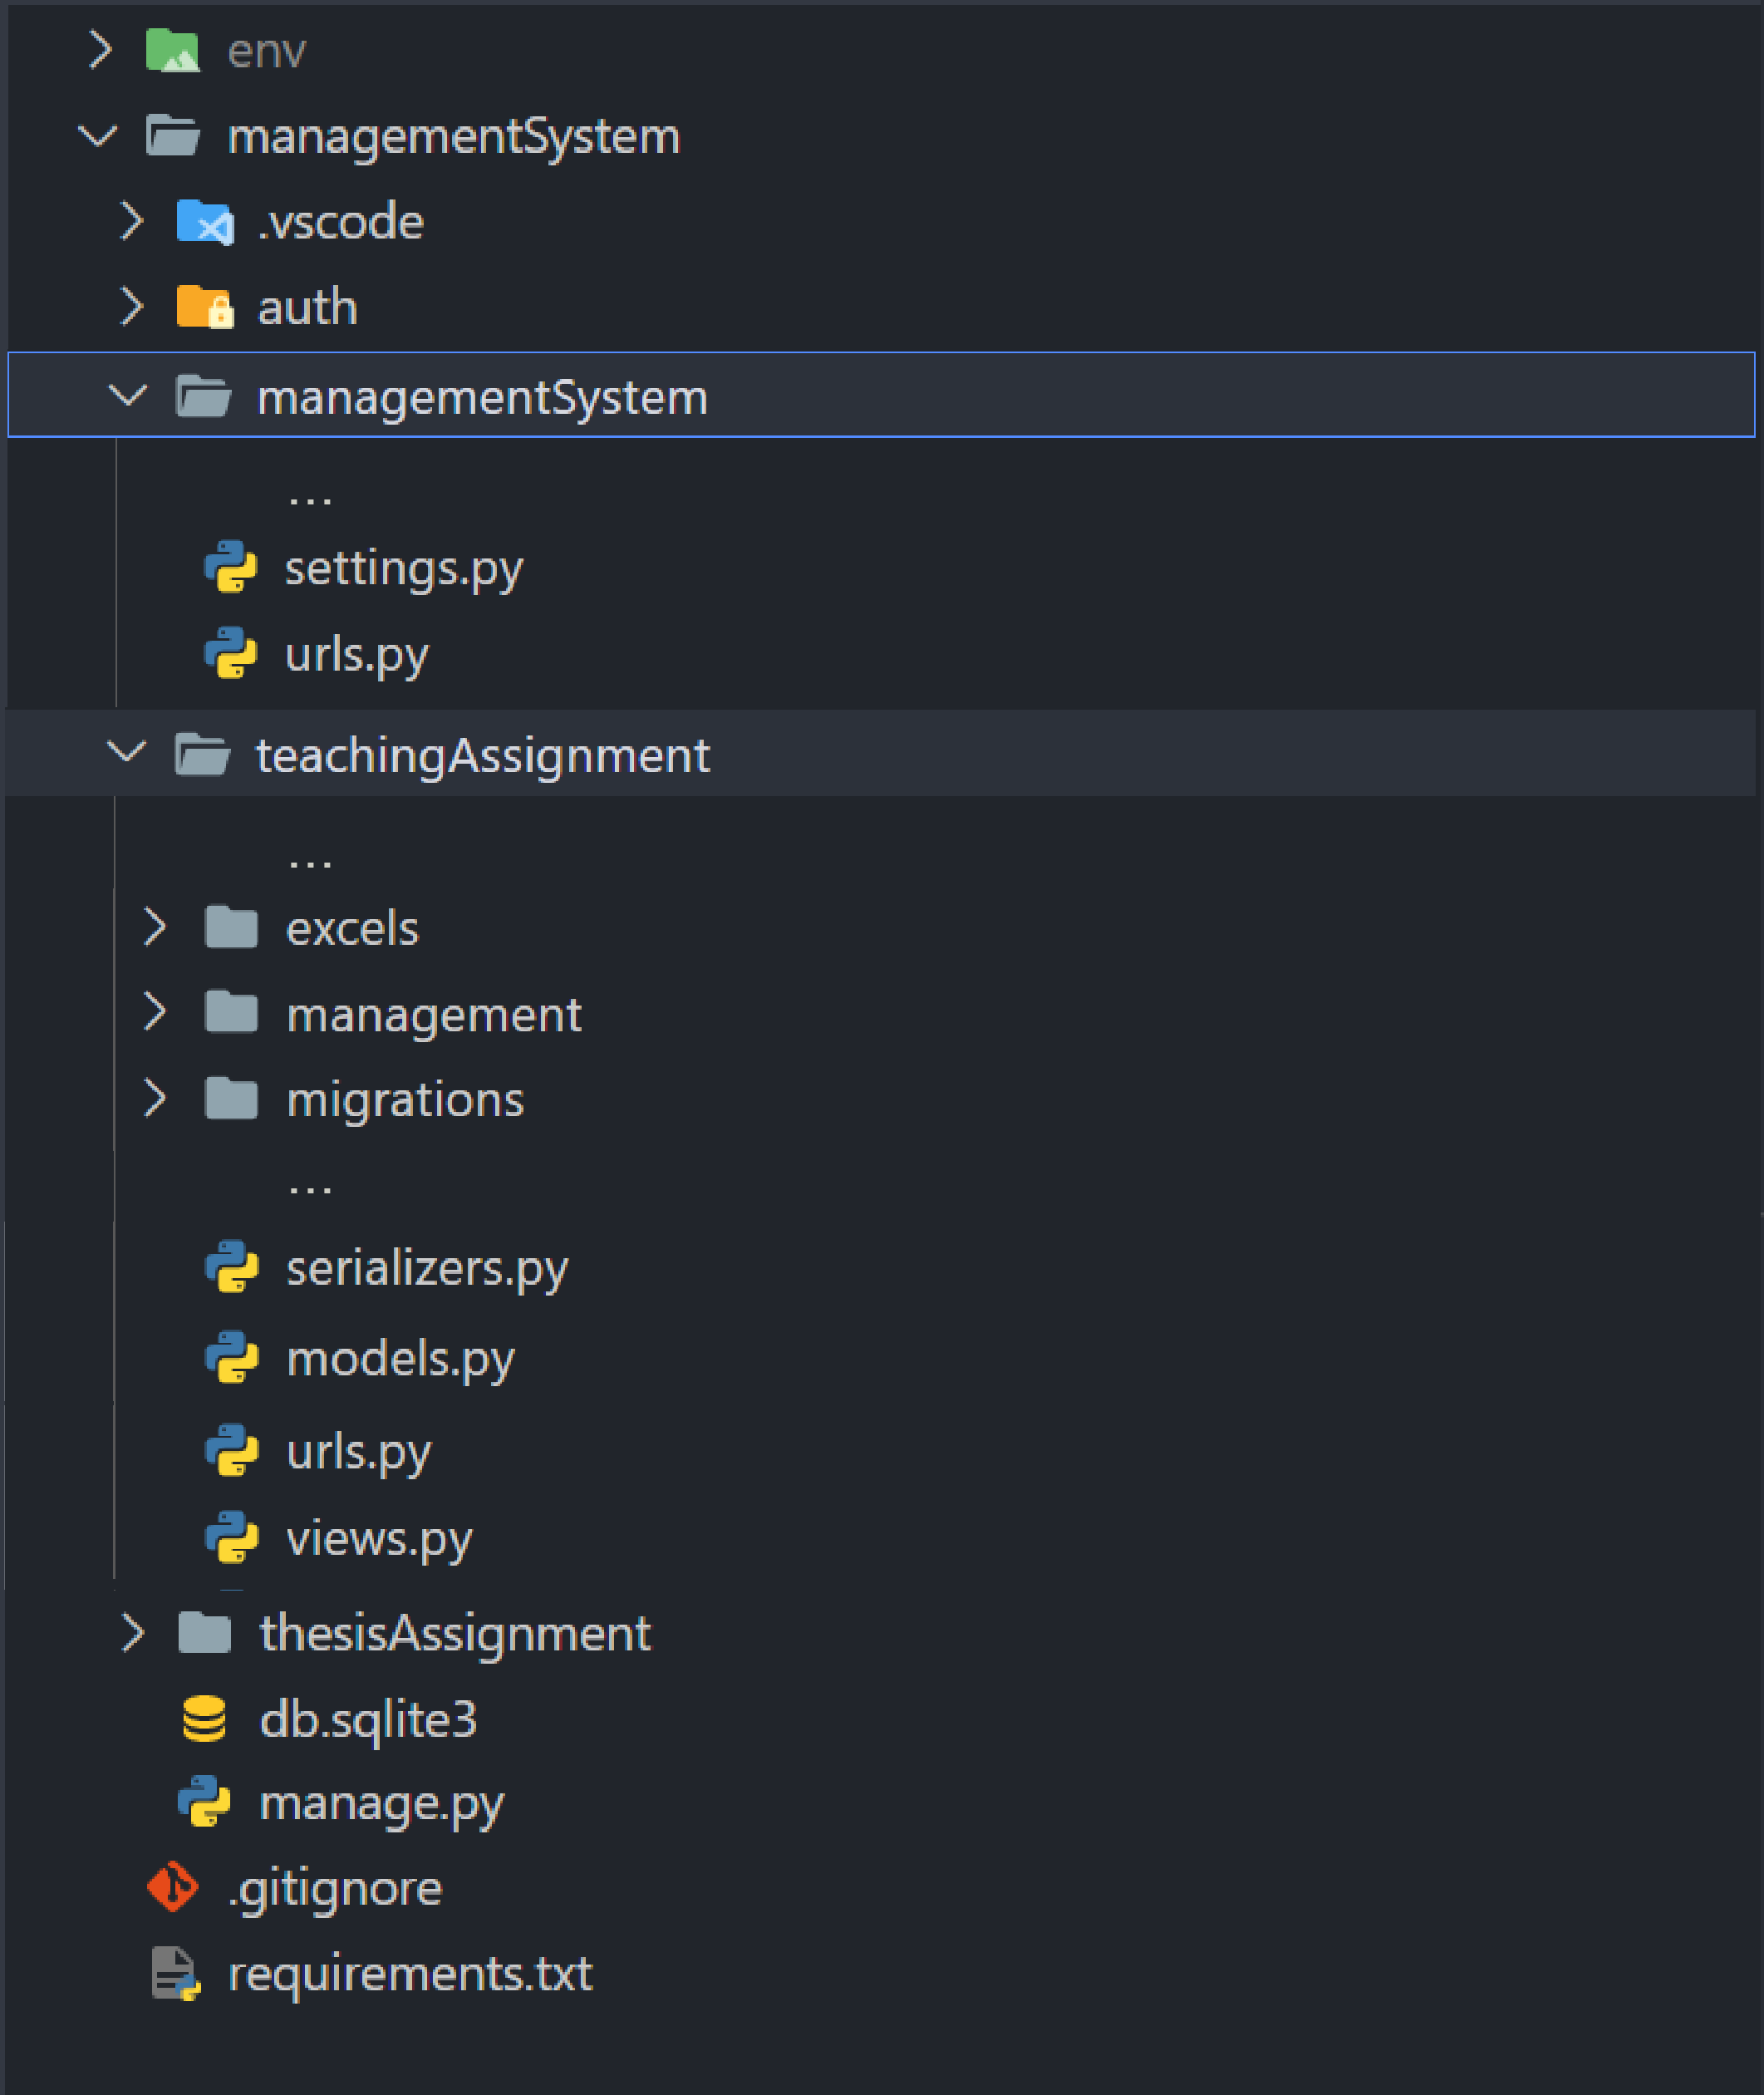
\includegraphics[scale=0.18]{Graphics/Extensibility/server-structure.png}
    \caption{Estructura de los ficheros del proyecto servidor}
    \label{img-server-structure}
\end{figure}

A continuación se describen las carpetas y ficheros principales del proyecto 
servidor.

\begin{itemize}
    \item \texttt{managementSystem}: es la carpeta principal del proyecto, en el fichero \texttt{settings.py} se encuentran
    todas las configuraciones. En el fichero \texttt{url.py} se deben agregar las \textit{urls} de las \textit{apps} creadas 
    en el proyecto. En este caso, se incluyen las \textit{urls} de las \textit{apps} \texttt{teachingAssignment} y \texttt{teachingAssignment}. 
    \item \texttt{teachingAssignment}:  \textit{app} creada para el desarrollo del proceso de asignación de docencia. En la carpeta \texttt{excels}  
    se implementó la funcionalidad de descargar un fichero CSV con la información de la asignación de docencia. 
    \item \texttt{thesisAssignment}:  \textit{app} creada para el desarrollo del proceso de planificación de las tesis. En la carpeta \texttt{excels} 
    se implementó la funcionalidad de descargar en ficheros CSV la información de los tribunales y defensas de tesis.
    \item \texttt{teachingAssignment/management}: en esta carpeta se encuentran las implementaciones de los comandos \texttt{save\_database} 
    y \texttt{fill\_database}, con los que se permite salvar y poblar la base de datos, respectivamente.
\end{itemize}


Para el desarrollo del cliente se utilizó la biblioteca Quasar. El proyecto 
cliente se creó con el uso de la herramienta Quasar CLI. 
La distribución de los ficheros quedó como se muestra a continuación.

\begin{figure}[H]
    \centering
    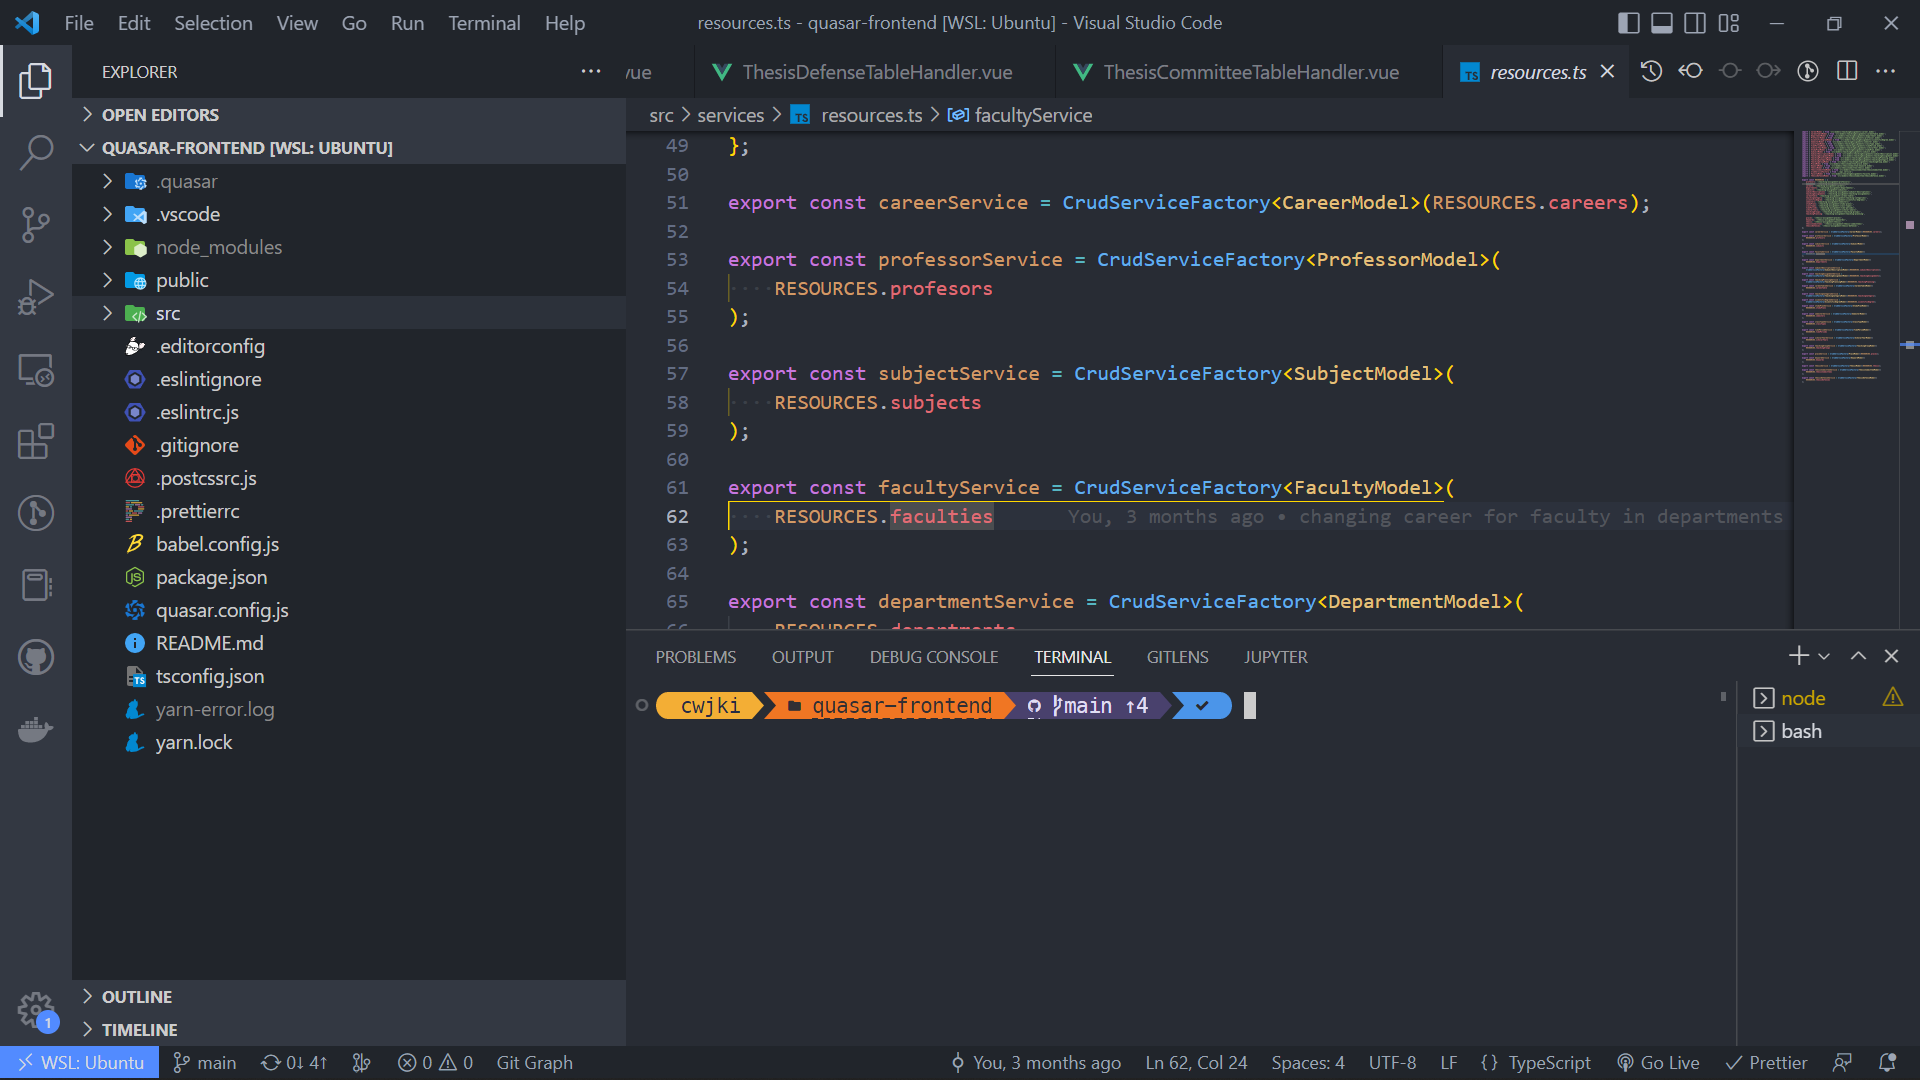
\includegraphics[scale=0.65]{Graphics/Extensibility/client-structure.png}
    \caption{Estructura de los ficheros del proyecto servidor}
    \label{img-client-structure}
\end{figure}

Todo el desarrollo del cliente se encuentra dentro de la carpeta \texttt{src}.
A continuación se describe qué encontrar en cada una de las carpetas.

\begin{itemize}
    \item \texttt{assets}: las imágenes que se utilizaron en el proyecto.
    \item \texttt{boot}: configuraciones que se desean inyectar antes de que se cree una instancia de la componente 
    raíz de la aplicación. Por ejemplo, configurar la \textit{url} base para la comunicación con el servidor. 
    \item \texttt{components}: las componentes implementadas para el funcionamiento del proyecto. 
    Por ejemplo, en este trabajo se implementó una componente genérica para la visualización de cada una de las entidades 
    que intervienen en los procesos de asignación de docencia y planificación de las tesis.  
    \item \texttt{css}: los ficheros relacionados con el estilo utilizado. Por ejemplo, se redefinieron los colores 
    \texttt{primary} y \texttt{secondary} por los colores que aparecen en el logo de MATCOM. 
    \item \texttt{hooks}: los \textit{hooks} que se implemetaron para el funcionamiento del proyecto.
    Por ejemplo, se creó un \textit{hook} para conocer qué departamento se desea administrar en cada momento 
    y mostrar solo los datos relacionados con ese departamento.
    \item \texttt{layouts}: la implementación de la barra de navegación principal.
    \item \texttt{models}: las definiciones de los tipos utilizados. Por ejemplo, se creó una interfaz \texttt{ProfessorModel} donde se definen los 
    campos que tiene un profesor, como: \texttt{id}, \texttt{name}, \texttt{lastName}, \texttt{department}, \texttt{scientificDegree} y \texttt{teachingCategory}.  
    \item \texttt{pages}: la implementación de las páginas de la aplicación web.
    \item \texttt{router}: el enrutamiento de la aplicación web.
    \item \texttt{services}: la implementación de una capa de abstracción para la comunicación con el servidor.
\end{itemize}


Se definió una capa de abstracción para la comunicación con 
el servidor que permite, a partir de una \textit{url}, realizar las operaciones CRUD: \textit{create}, \textit{read}, \textit{update}, \textit{delete}. 
A continuación se muestra su definición.



\begin{verbatim}
    export const CrudServiceFactory = <T = any>(url: string) => {
    return {
        url: url,
        fullUrl: baseURL + url,
        create(obj: T) {
            return api.post<T>(url, obj);
        },
        list(query: Dictionary = {}) {
            return api.get<ListResult<T>>(url + buildQuery(query));
        },
        update(id: string, obj: Dictionary) {
            return api.patch<T>(url + id + '/', obj);
        },
        delete(id: string) {
            return api.delete<T>(url + id);
        },
    };
};
\end{verbatim}


En el fichero \texttt{resources.ts}, que se encuentra dentro de la carpeta \texttt{services},
se debe definir un servicio para cada uno de los \textit{endpoints}  
con los que se quiera realizar la comunicación. Por ejemplo,
para realizar las peticiones relacionadas a los profesores se 
creó el servicio \texttt{professorService}, cuya definición se muestra a continuación.

\begin{verbatim}
    export const RESOURCES = {
        profesors: '/teaching-assignment/professors/',
        faculties: '/teaching-assignment/faculties/',
        careers: '/teaching-assignment/careers/',
        ...,

    };

    export const professorService = CrudServiceFactory<ProfessorModel>(
        RESOURCES.profesors
    );
\end{verbatim}


De esta forma, desde cualquier fichero que se importe el servicio \texttt{professorService},
se pueden realizar peticiones al servidor del estilo:

\begin{verbatim}
    professorService.create(obj: T)
    professorService.list(query: Dictionary)
    professorService.update(id: string, obj: Dictionary)
    professorService.delete(id)
\end{verbatim}


Desde la aplicación web cliente se pueden visualizar y modificar todos los 
datos que intervienen en los procesos que se informatizaron.
Para ello, se creó una página para administrar los 
datos de cada una de las entidades que se modelaron en la base de datos.
Se implementó una componente genérica que a partir de una configuración
transforma los datos que se reciben desde el servidor y los muestra en una tabla.
En esta tabla genérica se implementaron las operaciones \textit{create}, \textit{delete} y \textit{update}. 
A continuación se muestra la interfaz que define una configuración para esta  
tabla.

\begin{verbatim}
    export interface GenericCrudTableConfig {
        name: string;
        singularLabel: string;
        searchLabel?: string;
        actions?: {
            create?: boolean;
            update?: boolean;
            delete?: boolean;
            external?: {
                color: string;
                icon: string;
                func: () => void;
            }[];
        };
        service: CRUDService;
        query?: Dictionary;
        fields: FieldModel[];
        defaultValues?: Dictionary;
    }
\end{verbatim}

En el campo \texttt{actions} se debe especificar si se desean 
habilitar las operaciones \textit{create}, \textit{delete} o \textit{update}.
En el campo \texttt{services} se debe especificar el servicio
a partir del cual se va a poblar la tabla, 
por ejemplo, el \texttt{professorService} que se describió anteriormente,
y en el campo \texttt{fields} se deben definir los datos que se deseen mostrar
a partir de los objetos que se reciben con el servicio especificado.

A continuación se ilustra un ejemplo de cómo configurar 
una tabla para administrar los departamentos.

\begin{verbatim}
<template>
    <generic-crud-data-table :config="config" />
</template>

<script lang="ts">
import { facultyService, departmentService } from 'src/services';

export default defineComponent({
    components: { GenericCrudDataTable },
    name: 'departmentHandler',
    props: {},
    emits: [],
    setup(props, { emit }) {
        const config = ref<GenericCrudTableConfig>({
            name: 'Departamentos',
            singularLabel: 'Departamento',
            searchLabel: 'Departamento o Facultad',
            service: departmentService,
            fields: [
                {
                    name: 'name',
                    label: 'Departamento',
                    type: 'text',
                },
                {
                    name: 'faculty',
                    label: 'Facultad',
                    column: {
                        transform(row) {
                            return `${row.faculty.name}`;
                        },
                    },
                    type: 'select',
                    selectOptions: {
                        list: facultyService.list,
                        value: 'id',
                        label: 'name',
                    },
                    rules: ['required'],
                },
            ],
            actions: {
                create: true,
                update: true,
                delete: true,
            },
        });

        return { config };
    },
});
</script>

\end{verbatim}

En este caso se define que el servicio a partir del cual se 
va a poblar la tabla es \texttt{departmentService}, en \texttt{fields}
se especifica que los campos que se desean 
mostrar son el nombre del departamento y la facultad a la que pertenece, y en 
\texttt{actions} que se desean habilitar las operaciones 
de \textit{create}, \textit{update} y \textit{delete} en la tabla. En la 
figura \ref{cap5-table-department} se muestra el resultado de esta configuración.

\begin{figure}[H]
    \centering
    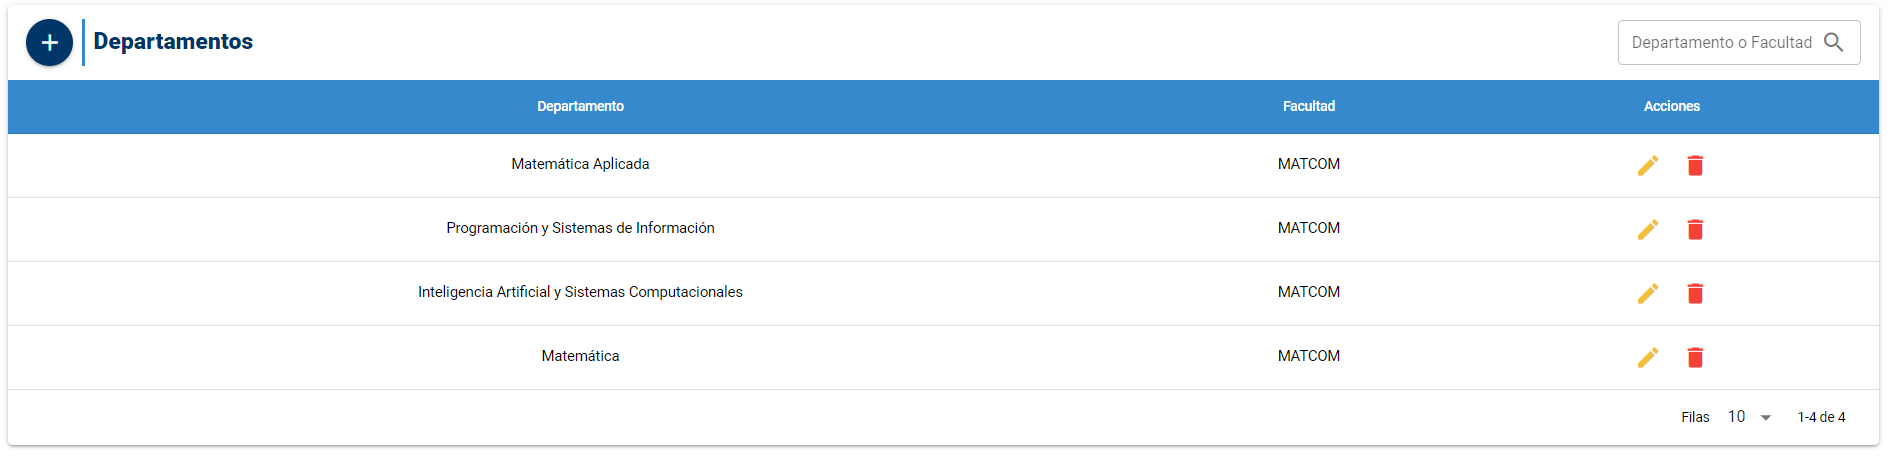
\includegraphics[scale=0.3]{Graphics/Extensibility/department-table.png}
    \caption{Tabla para los departamentos}
    \label{cap5-table-department}
\end{figure}


Si se desea extender este concepto para administrar los datos que intervienen
en los procesos que se agregen en el sistema,
solo se debe utilizar la componente \texttt{genericCrudDataTable}
y definir la configuración que tendrá la tabla.

% La componente \texttt{genericCrudDataTable} recibe una configuración, por tanto 
% si se desea reutilizar esta componente para administrar los datos que intervienen en los 
% procesos que se agreguen al sistema, solo se debe definir la configuración de la tabla.


En la siguiente sección, se recomiendan las pautas a seguir para la incorporaración 
de nuevos procesos en el sistema de gestión.

\section{Recomendaciones para agregar un nuevo proceso en el sistema de gestión}\label{cap5:recommendations}
Para describir los pasos que se recomiendan seguir para agregar un nuevo proceso en el sistema,
se ilustrará con el proceso de planificación de las tesis. Supongamos que en el 
sistema de gestión solo está informatizado el proceso de asignación de docencia y se 
quiere agregar el de planificación de las tesis.

En el lado del servidor,
se recomienda crear una una \textit{app} de Django para encapsular los ficheros necesarios 
que intervienen en la modelación del proceso de planificación de las tesis.
Por tanto el primer paso sería ejecutar el siguiente comando.

\begin{verbatim}
    python manage.py startapp thesisAssignment
\end{verbatim}

Dentro de la carpeta \texttt{thesisAssignment} se deben definir los modelos, serializadores, 
vistas y urls necesarias. Para el proceso de planificación de las tesis se crearon nuevas 
entidades como \texttt{Place}, \texttt{Keyword}, \texttt{Thesis}, \texttt{ThesisCommittee} y \texttt{ThesisDefense}. 
Se modelaron sus relaciones, incluso con otras entidades que se habían definido durante el proceso de asignación de 
docencia. Por ejemplo, entre las entidadades \texttt{Thesis} y \texttt{Professor} se definieron las relaciones de tutor y cotutor. \\


En el lado del cliente, se siguieron los siguientes pasos para agregar el proceso 
de planificación de las tesis. 

\begin{itemize}
    \item Se creó la carpeta \texttt{thesisCommittee}, dentro de la carpeta \texttt{src}/models, para 
    definir los tipos de las entidades que interviene en este proceso. Se agregaron las interfaces 
    \texttt{KeywordModel}, \texttt{PlaceModel}, \texttt{ThesisModel}, \texttt{ThesisCommitteeModel} y \texttt{ThesisDefenseModel}.
    \item En el fichero \texttt{resources.ts}, que se encuentra en la carpeta \texttt{services}, se crearon los servicios 
    para realizar las peticiones al servidor:
    \texttt{placeService}, \texttt{keywordService}, \texttt{thesisService}, \texttt{thesisCommitteeService} y \texttt{thesisDefenseService}.
    \item Se creó una carpeta \texttt{thesisCommittee} dentro de la carpeta \texttt{src/components/tables} para agrupar 
    las componentes que se definen las configuraciones de las tablas correspondientes 
    a este proceso.
    \item Se creó una carpeta \texttt{thesisCommittee} dentro de la carpeta \texttt{src/pages} para agrupar 
    las vistas necesarias para la modelación de este proceso: \texttt{Keywords.vue}, \texttt{Place.vue}, 
    \texttt{Thesis.vue}, \texttt{ThesisCommittee.vue} y \texttt{ThesisDefense.vue}.
    \item En el fichero \texttt{routes.ts} que se encuentra en la carpeta \texttt{src/routes}, 
    se agregaron las rutas que llevan a las vistas definidas en el paso anterior.
    \item Se agregaron los botones a la barra de navegación que permiten ir a las vistas que se crearon 
    en este proceso.
\end{itemize}


En resumen, en el lado del servidor, se recomienda la creación de una nueva \textit{app} de Django que agrupe los ficheros necesarios para la modelación del 
proceso que se desea incorporar en el sistema. Se deben definir los modelos, cómo se serializan los datos y a través de cuáles \textit{urls} se exponen.
En el lado del cliente se recomienda definir los tipos de los datos que se van a recibir, los servicios necesarios para realizar 
las peticiones al servidor, agrupar las componentes y las vistas necesarias en carpetas que indiquen el proceso que se está informatizando y agregar un mecanismo para 
acceder a esas vistas. 

% Supongamos que se quiere agregar al sistema de gestión el proceso de planificación de 
% las evaluaciones de un semestre. A continuación se describen los pasos principales
% que se sugieren para la integración de este proceso.

% \begin{itemize}
%     \item Crear una nueva app de django con el comando tal.
%     \item Dentro de la carpeta creada en el paso anterior definir los modelos, serializadores, 
%     vistas y urls necesarios en ficheros nombrados models.py, serializers.py, views.py, urls.py respectivamente. 
%     \item Crear una carpeta con el nombre del proceso que se está modelando dentro de las carpetas pages y components. 
%     En la carpeta pages se encuentrar las vistar principales y dentro de la carpeta components definir las componentes 
%     necesarias 
%     \item En la carpeta services se implemetó una api para la comunicación con el servidor. Se creo un CRUDServiceFactory 
%     que permite realizar pedidos de crear, listar, actualizar y borrar. Solo se necesita agregar la url y el tipo de dato 
%     en el fichero resources. 
    

% \end{itemize}



